\documentclass[border=20pt]{standalone}
\usepackage[american]{circuitikz}
\usepackage{amsmath}%To allow \cfrac macro
\usepackage{bm}%Bold math
\usetikzlibrary{arrows.meta,decorations.markings}

\begin{document}
    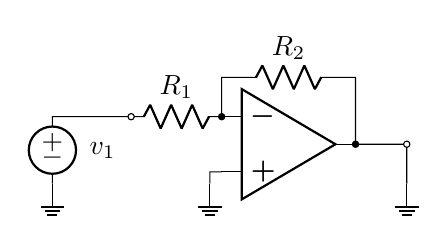
\begin{tikzpicture}
\ctikzset{bipoles/length=1cm}
\draw
(0, 0) node[op amp] (opamp) {}
(opamp.-) to[R,l_=$R_1$,-o] (-2, 0.35) -- (-3, 0.35) to [V=$v_1$] (-3,-0.5) to (-3,-0.5) node[ground]{}
(opamp.-) to[short,*-] ++(0,0.5) coordinate (leftC)
to[R=$R_2$] (leftC -| opamp.out)
to[short,-*] (opamp.out) to [short,-o] (1.5,0) to (1.5,-0.5) node[ground]{}
(opamp.+) -- (-1,-0.35) to (-1,-0.5) node[ground]{};
    \end{tikzpicture}
\end{document}